\documentclass{article}
\usepackage[UTF8, scheme = plain]{ctex}
\usepackage{amsmath,amsfonts,amsthm,amssymb,amssymb,amsfonts}
\usepackage{setspace}
\usepackage{fancyhdr}
\usepackage{lastpage}
\usepackage{extramarks}
\usepackage{chngpage}
\usepackage{soul,color}
\usepackage{graphicx,float,wrapfig}
\usepackage{CJKutf8}
\usepackage{graphicx}
\usepackage[noend]{algpseudocode}
\usepackage{algorithmicx,algorithm}
\usepackage{listings}
\newcommand{\Class}{人工智能导论}
%\newcommand{\ClassInstructor}{Jian Li}%

% Homework Specific Information. Change it to your own
\newcommand{\Title}{拼音输入法}
%\newcommand{\DueDate}{Oct 12, 2022}
\newcommand{\StudentName}{周韧平}
\newcommand{\StudentClass}{计 11}
\newcommand{\StudentNumber}{2021010699}

% In case you need to adjust margins:
\topmargin=-0.45in      %
\evensidemargin=0in     %
\oddsidemargin=0in      %
\textwidth=6.5in        %
\textheight=9.0in       %
\headsep=0.25in         %

% Setup the header and footer
\pagestyle{fancy}                                                       %
\lhead{\StudentName}                                                 %
\chead{\Title}  %
\rhead{\firstxmark}                                                     %
\lfoot{\lastxmark}                                                      %
\cfoot{}                                                                %
\rfoot{Page\ \thepage\ of\ \protect\pageref{LastPage}}                          %
\renewcommand\headrulewidth{0.4pt}                                      %
\renewcommand\footrulewidth{0.4pt}                                      %

%%%%%%%%%%%%%%%%%%%%%%%%%%%%%%%%%%%%%%%%%%%%%%%%%%%%%%%%%%%%%
% Some tools
\newcommand{\enterProblemHeader}[1]{\nobreak\extramarks{#1}{#1 continued on next page\ldots}\nobreak%
                                    \nobreak\extramarks{#1 (continued)}{#1 continued on next page\ldots}\nobreak}%
\newcommand{\exitProblemHeader}[1]{\nobreak\extramarks{#1 (continued)}{#1 continued on next page\ldots}\nobreak%
                                   \nobreak\extramarks{#1}{}\nobreak}%

\newcommand{\homeworkProblemName}{}%
\newcounter{homeworkProblemCounter}%
\newenvironment{homeworkProblem}[1][Problem \arabic{homeworkProblemCounter}]%
  {\stepcounter{homeworkProblemCounter}%
   \renewcommand{\homeworkProblemName}{#1}%
   \section*{\homeworkProblemName}%
   \enterProblemHeader{\homeworkProblemName}}%
  {\exitProblemHeader{\homeworkProblemName}}%

\newcommand{\homeworkSectionName}{}%
\newlength{\homeworkSectionLabelLength}{}%
\newenvironment{homeworkSection}[1]%
  {% We put this space here to make sure we're not connected to the above.

   \renewcommand{\homeworkSectionName}{#1}%
   \settowidth{\homeworkSectionLabelLength}{\homeworkSectionName}%
   \addtolength{\homeworkSectionLabelLength}{0.25in}%
   \changetext{}{-\homeworkSectionLabelLength}{}{}{}%
   \subsection*{\homeworkSectionName}%
   \enterProblemHeader{\homeworkProblemName\ [\homeworkSectionName]}}%
  {\enterProblemHeader{\homeworkProblemName}%

   % We put the blank space above in order to make sure this margin
   % change doesn't happen too soon.
   \changetext{}{+\homeworkSectionLabelLength}{}{}{}}%

\newcommand{\Answer}{\ \\\textbf{Answer:} }
\newcommand{\Proof}{\ \\\textbf{Proof:} }
\newcommand{\Acknowledgement}[1]{\ \\{\bf Acknowledgement:} #1}
\newcommand{\D}{\text{ d}}

%%%%%%%%%%%%%%%%%%%%%%%%%%%%%%%%%%%%%%%%%%%%%%%%%%%%%%%%%%%%%
\lstset{ %
	language=C++,                % choose the language of the code
	basicstyle=\fontspec{Consolas},       % the size of the fonts that are used for the code
	%numbers=left,                   % where to put the line-numbers
	numberstyle=\footnotesize,      % the size of the fonts that are used for the line-numbers
	stepnumber=1,                   % the step between two line-numbers. If it is 1 each line will be numbered
	numbersep=5pt,                  % how far the line-numbers are from the code
	backgroundcolor=\color{white},  % choose the background color. You must add \usepackage{color}
	showspaces=false,               % show spaces adding particular underscores
	showstringspaces=false,         % underline spaces within strings
	showtabs=false,                 % show tabs within strings adding particular underscores
	frame=single,           % adds a frame around the code
	tabsize=2,          % sets default tabsize to 2 spaces
	captionpos=b,           % sets the caption-position to bottom
	breaklines=true,        % sets automatic line breaking
	breakatwhitespace=false,    % sets if automatic breaks should only happen at whitespace
	escapeinside={\%*}{*)}          % if you want to add a comment within your code
}

%%%%%%%%%%%%%%%%%%%%%%%%%%%%%%%%%%%%%%%%%%%%%%%%%%%%%%%%%%%%%
% Make title
\title{\textmd{\bf \Class: \Title}}
\author{\textbf{\StudentName}\ \ \StudentClass\ \ \StudentNumber}
%%%%%%%%%%%%%%%%%%%%%%%%%%%%%%%%%%%%%%%%%%%%%%%%%%%%%%%%%%%%%

\begin{document}
\begin{spacing}{1.1}
\maketitle \thispagestyle{empty}
%\cite{}
%%%%%%%%%%%%%%%%%%%%%%%%%%%%%%%%%%%%%%%%%%%%%%%%%%%%%%%%%%%%%
% Begin edit from here
\section{基本原理}
	\subsection{隐式马尔可夫模型}
	\hspace{1.4em} 拼音输入法的实现原理基于\textbf{隐马尔科夫模型(HMM)}。其中,\textbf{Viterbi算法}是HMM中的一种解码算法,用于寻找最有可能产生观测事件序列的维特比路径——隐含状态序列,特别是在马尔可夫信息源上下文和隐马尔可夫模型中。
	
	首先,我们需要定义一些概念。在HMM中,有两个序列:\textbf{观察序列}和\textbf{状态序列}。观察序列是我们可以观察到的数据,而状态序列是我们无法直接观察到的数据。在拼音输入法中,观察序列就是拼音序列,而状态序列就是汉字序列。具体来说,对于给定长度为n的拼音序列$O=o_1o_2\cdots o_n$,需要确定每一个单独的拼音$s_i$对应的字符$w_i$,使得中文序列 $W=w_1w_2\cdots w_n$ 最佳。
	
	利用现有的语料库,我们可以统计出在给定拼音串$O$的情况下字符串$W$匹配的概率$P(w)$,也即优化概率$P(w_1w_2\cdots w_n)$。而根据条件概率公式可以进一步拆分为$$P(w_1w_2\cdots w_n) = P(w_1)P(w_2|w_1)P(w_3|w_1w_2)\cdots P(w_n|w_1\cdots w_{n-1})$$
	\hspace{1.4em}
	等式两边取负对数后,也即最小化$$-\log(P(w_1w_2\cdots w_n)) = -\log(P(w_1))-\log(P(w_2|w_1))-\log(P(w_3|w_1w_2))\cdots -\log(P(w_n|w_1\cdots w_{n-1}))$$
	\hspace{1.4em}
	这里我们可以将$-\log(P(w_n|w_1\cdots w_{n-1}))$形象地理解为在给定拼音串$O$的情况下,$w_1\cdots w_{n-1}$到$w_n$的“距离”,将原问题转化为\textbf{求解最短路问题}。
	
	考虑到统计$P(w_n|w_1\cdots w_{n-1})$是一件很困难的事,我们引入m阶Markov模型,即第n个字出现的概率只和其前面m个字有关,用数学公式表示就是$P(w_n|w_1\cdots w_{n-1}) =P(w_n|w_{n-m}\cdots w_{n-1})$,在本次实验中,m取到了1,2,3,分别对应一、二、三元Markov模型。
	
	基于以上分析,我们的问题为求解最短路径
	$$\Sigma_{i=1}^nDistance(i)$$  
	\hspace{1.4em}
	定义$ Distance(w_n)=-\log(P(w_n|w_{n-m}\cdots w_{n-1}))$,当$n<m$时, $Distance(w_n)=-\log(P(w_n|w_0\cdots w_{n-1}))$
	
	\subsection{Viterbi算法}
	\hspace{1.4em}
	对于给定的字符串$S=s_1\cdots s_n$假设$W_i = \{w_{i,j}|j=1,2,\cdots\}$表示$s_i$拼音对应的所有汉字集合。定义$w_0,w_{n+1}$分别为初始和末尾状态。
	
	根据模型,求解最短路问题可以转化为\textbf{动态规划求解有向无环图的最短路问题},我们用表 \verb|distance[ind][cur]| 存储$s_{ind}$对应汉字$cur$的状态,该状态内有两个分量dist和before,dist记录从$w_0$到当前状态的最小距离,before指向最短路径上该节点的前驱。
	
	当某一刻已经确定从$W_0$到$W_i$中所有结点(也就是确定了图中某一列所有结点)的状态后,对于下一列的所有状态结点$cur = w_{i+1,j}$,存在\textbf{状态转移函数} \verb|distance[ind+1][cur] = min(distance[ind][cur]+| $Distance(w_n)$ \verb|)|,$\forall w_n \in W_n$ 其中$Distance(w_n)$为1.1节中定义的给定前m个汉字后到下一个汉字的距离,前m个汉字由已经确定的状态 \verb|distance[ind][cur]| 给出。
	
	\begin{figure}[h]
		\centering
		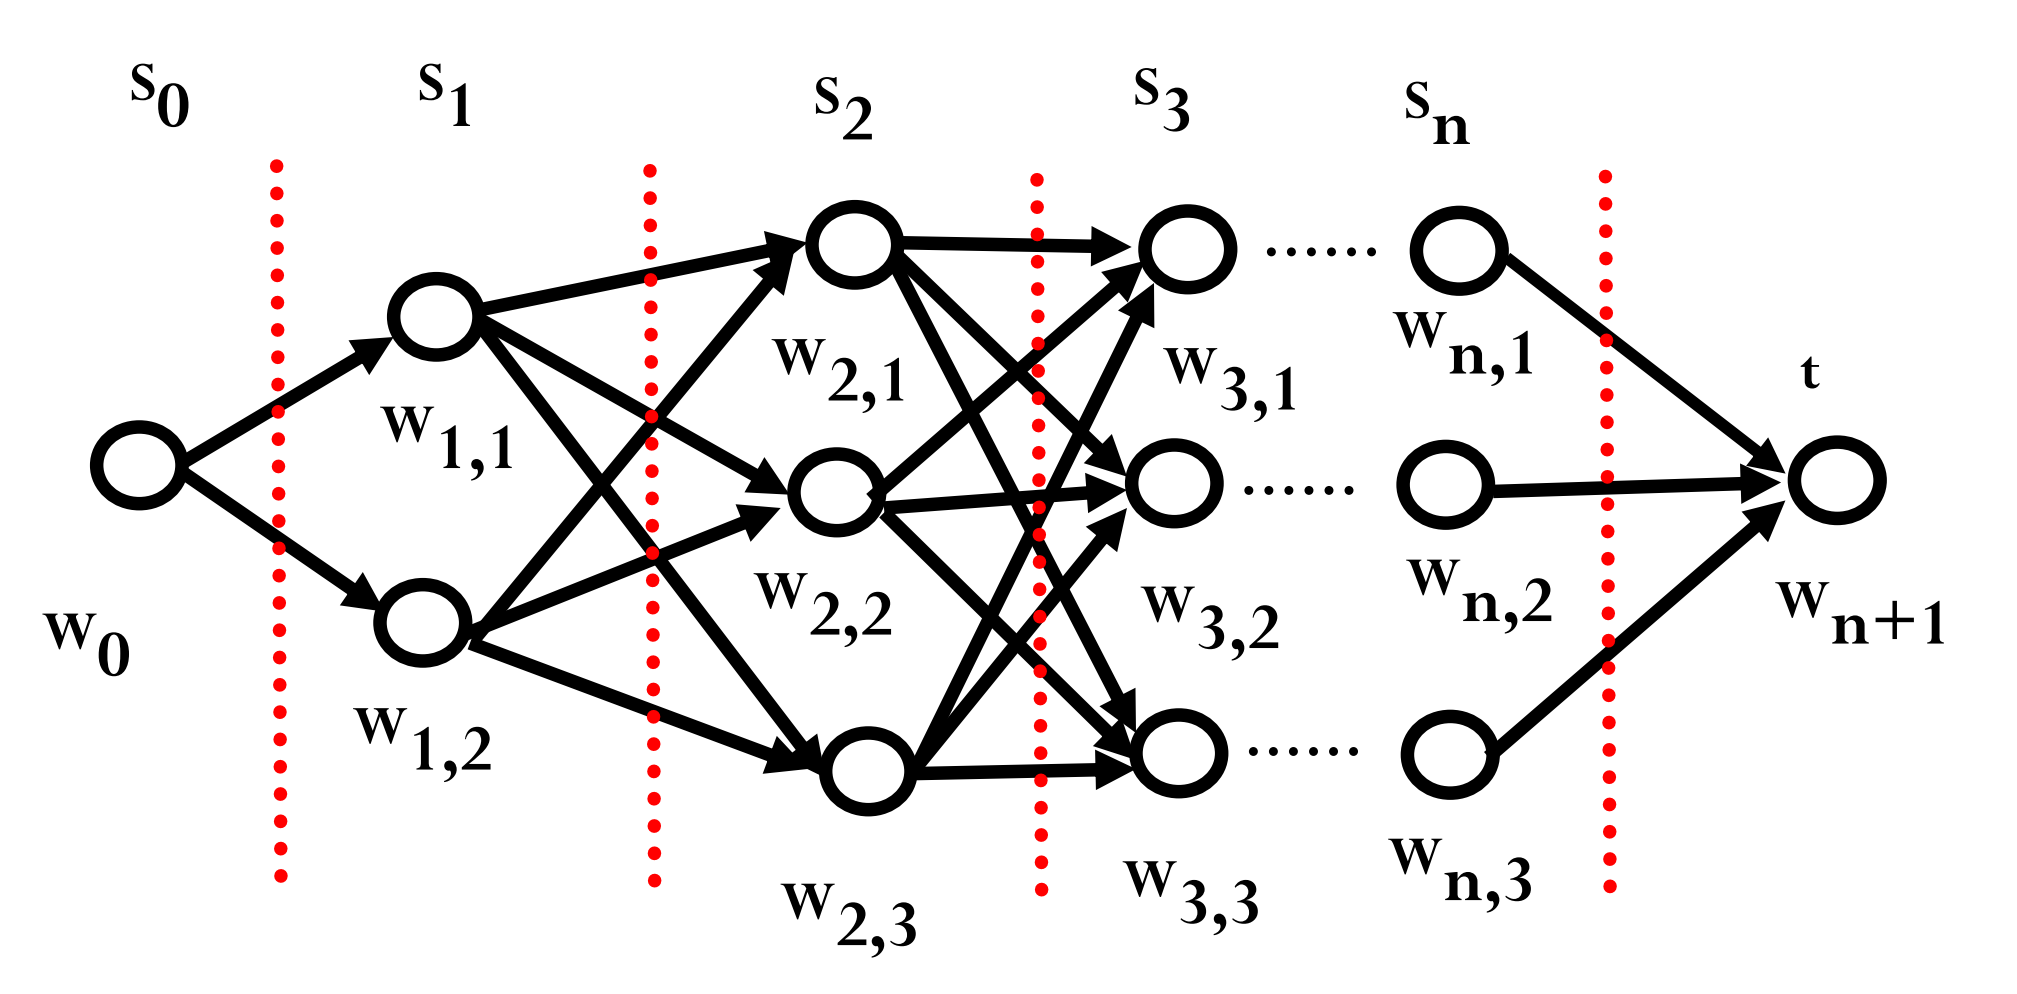
\includegraphics[width=0.8\linewidth]{pic/01.png}
		\caption{拼音转化为汉字的推断图模型}
	\end{figure}

\section{实验过程}
	\subsection{实验环境及项目结构}
	本实验在windows x86系统上进行,主要代码用 python 语言编写,用pip进行包管理,运行本程序需安装`json`、`re`、`os`、`tqdm`、`argpase`、`math`包。数据用 \verb|*.jsoon *.txt| 格式存储。项目整体结构如下:
	\begin{lstlisting}
	{
	|-data: 训练用的数据集
		|-input.txt:标准输入集
		|-output.txt:report中提到的最佳参数和模型下生成
		|-std_word_table.txt: 下发的拼音汉字对照表
		|-weibo2020_build_line.txt: 微博2020数据清洗后结果(新浪2016的数据清洗结果过大上传至网盘)
		|-sina:在三种测试集上新浪2016数据生成模型下的测试结果
			|-500line: 标准测试集
			|-poem: 诗歌测试集
			|-semetic: 感情类文本测试集
		|-weibo:在三种测试集上微博2020数据生成模型下的测试结果
			|-500line: 标准测试集
			|-poem: 诗歌测试集
			|-semetic: 感情类文本测试集
	|-src
		|-model: 训练生成的模型(微博2020,新浪2016)
			|-pinyin2word.json: 拼音到汉字表处理成json形式
			|-std_word_table.txt: 一二级汉字表
			|-word_dictionary_weibo2020:微博2020生成的词频表
				|-one_word_dict.json: 一元词频表
				|-two_word_dict.json: 二元词频表
				|-three_word_dict.json: 三元词频表
				|-four_word_dict.json: 四元词频表
			|-word_dictionary_xinlang2016:新浪2016生成的词频表
				|-one_word_dict.json: 一元词频表
				|-two_word_dict.json: 二元词频表
				|-three_word_dict.json: 三元词频表
				|-four_word_dict.json: 四元词频表
		|-utils.py: 数据清理工具
		|-train.py: 训练生成模型
		|-viterbi.py: 隐式Markov模型主体算法
		|-README.md: 项目说明文件
		
	}
	\end{lstlisting}
	\subsection{语料获取与处理}
	\hspace{1.4em}
	本实验中我分别选取了助教提供的\textbf{新浪新闻2016年的新闻语料}和\textbf{微博2020年发布的情绪分类技术评测}两个语料库来构建模型。二者语料规模分别为\textbf{亿级}和\textbf{百万级}(字)通常来说,,在不考虑其它条件下,程序的预测准确率一般和语料库规模正相关,因此下面在展示准确率和测试结果时除做特殊说明外,均为新浪新闻语料库训练得到的模型,微博语料库仅做语料库效果对比时使用。
	
	语料库以txt格式存储在 \verb|\data\<语料库名称>| 文件夹下,处理数据时首先逐行读取txt中的内容并转换为json格式,提取有效键值后得到一条句子,作为中间结果存入 \verb|\data\<语料库名称_build_line.txt>| 中,此处为记录句子开始和结束的信息,读取每行后都会在收尾加入定界符(由于本实验最多只处理到四元模型,因此选择在首位添加三个句号,这样确保每个读到的汉字的后面和前面都有至少三个字符),这部分代码保存在 \verb|utils.py| 中,可以通过 \verb|python utils.py --data_type=<sina or weibo> --path=<path to data>| 来运行,该文件还写有 \verb|build_pinyin_word_dict| 函数,用来建立拼音到一二级汉字的映射表
	
	\subsection{构建词频表}
	\hspace{1.4em}
	得到纯文本数据后,下一步是根据数据建立词频表,下面以二元模型为例,解释构建词频表的结构:
	\begin{lstlisting}
{"前置字":{"count":xxx,"begin":xxx,"end":xxx,"后置字1":xxx,"后置字2":xxx,"后置字3":xxx}...
}
	\end{lstlisting}
	每个字段含义如下:
	\begin{itemize}
		\item 前置字:二元字组中出现在第一个位置的字
		\item 后置字:二元组出现在第二个位置的字
		\item count:前置字出现的总次数
		\item begin:前置字出现在一个分句的开头的次数(定义一个分句为由中文标点符号分隔的句子)
		\item end:前置字出现在一个分局末尾的次数
	\end{itemize}
	
	\hspace{1.4em}
	逐个扫描文本,每当读入一个一二级汉字时,读取词典中对应键值的数据,并根据下一个是一二级汉字/非一二级汉字,将对应键值的 汉字/end 加一,同时根据其前一个位置是否为标点符号来决定是否将 begin 键值加1,无论何种情况,均将 count 键值加一
	
	一、三、四元词频表采用相似的方法建立,区别在于嵌套词典的层数,此外,begin/end 的信息只需记录一次即可,为了提高数据处理速度,仅在二元词表中记录此信息
	
	相关代码保存在 \verb|train.py| 中,可以通过 \verb|python train.py --data_type=<1/2/3/4> --path=<path to data>| 来运行,运行后得到\verb|<one/two/three/four>_word_dict.json|文件,存储在根目录下
	
	\subsection{HMM推断过程}
	在定义的HMM类中,各种概率的计算规则如下:
	\begin{itemize}
		\item 初始概率:$P(w_1|w_0) = \frac{begin(w_1)}{count(w_1)}$
		\item 一元模型转移概率 $P(w_n|w_1w_2\cdots w_{n-1}) =P(w_n) =\frac{count(w_n)}{\Sigma_{w\in W_n} count(w)}$
		\item 二元模型转移概率 $P(w_n|w_1w_2\cdots w_{n-1}) =P(w_n|w_{n-1}) =\frac{count(w_{n-1}w_n)}{\Sigma_{w\in W_n} count(w_{n-1}w)}$
		\item 三元模型转移概率 $P(w_n|w_1w_2\cdots w_{n-1}) =P(w_n|w_{n-1}) =\frac{count(w_{n-2}w_{n-1}w_n)}{\Sigma_{w\in W_n} count(w_{n-2}w_{n-1}w)}$
		\item 四元模型转移概率 $P(w_n|w_1w_2\cdots w_{n-1}) =P(w_n|w_{n-1}) =\frac{count(w_{n-3}w_{n-2}w_{n-1}w_n)}{\Sigma_{w\in W_n} count(w_{n-3}w_{n-2}w_{n-1}w)}$ 	
	\end{itemize}
	为了防止概率过小出现精度爆炸,对所有概率取负对数,同时这样做也可以将所有乘法运算转化成加法运算,提高运算效率并防止溢出。
	
	\hspace{1.4em}
	
	推断时,首先根据首字的初始概率计算$w_0$到$w_1$的距离,然后根据转移概率递推n层至$w_{n+1}$,选出最短路径后输出结果。
	
	HMM类实现在\verb|viterbi.py|中,可运行 \verb|python viterbi.py --mode=<run/test> --model_path=<path to model>| 来推断,共有两种模式可以选择,run模式为手动输入拼音进行转换,test模式为运行指定测试样例并计算准确率。
	
	\subsection{算法优化}
	\subsubsection{引入结尾概率}
	\hspace{1.4em}
	受初始概率启发,尝试用结尾概率将句子末尾的信息添加至推断图中,即图中$w_n$到$w_{n+1}$的边权,其概率计算公式为$P(w_{n+1}|w_n) = \frac{end(w_n)}{count(w_n)}$
	\subsubsection{优化最小概率}
	\hspace{1.4em}
	对于不存在的字组合,一开始我将其边权定义为 \verb|float("inf")|,但这样做会导致生僻词出现时相应推断路径上被inf锁死,这在推断很多诸如专有名词之类等生僻词时会导致正确率大大降低。因此,当遇到不存在的字组合时,改为返回一个最小概率(如1e-6)避免被锁死的情况发生。
	\subsubsection{模型加权融合}
	\hspace{1.4em}
	为了达到更高的准确率,尝试在求转移概率时对一二三四元模型进行加权融合,其数学公式为$$P(w_n|w_{n-m}\cdots w_{n-1}) = c_0P(w_n)+c_1P(w_n|w_{n-1}) +  c_2P(w_n|w_{n-2}w_{n-1})+c_3P(w_n|w_{n-3}w_{n-2}w_{n-1})$$
	\hspace{1.4em}
	从语言的角度来理解就是将前4个字对下一个字的影响进行加权调整,尽量让下一个字能够充分得到前文语义。

\section{实验结果与分析}
	\subsection{模型加权融合}
	\hspace{1.4em}
	系数选取$c_0=0.01,\ c_1=1.61/0,\ c_2=7.8/0,\ c_3=0.1/0$,各种模型融合下预测准确率
	\begin {center}
	\begin{tabular}{|c|c|c|}
		\textbf{模型} & \textbf{字准确率} & \textbf{句准确率}\\
		\hline
		一元 & 56.67\% & 1.00\% \\
		\hline
		一、二元  & 82.06\% & 28.74\%\\
		\hline
		一、二、三元 & 90.93\% & 56.88\% \\
		\hline
		一、二、三、四元 & 90.96\% & 57.08\% \\
	\end{tabular}
	\end{center}
	\hspace{1.4em}
	\textbf{经过实验,在$c_0=0,\ c_1=1.61,\ c_2=7.8,\ c_3=0$ 条件下,拼音输入法的多元模型字准确率和行准确率可达到 92.31\% 与 64.87\% 。}
	\\\textbf{结果分析:}
	\begin{itemize}
		\item 尽管一元模型思路较为简单,但仅从字准确率来看也并不是一无是处,也可以达到一半以上的准确率
		\item 二三元模型在提升字准确率和句准确率上都有比较显著的效果,仅仅从效果来看,三元模型已经可以达到比较让人满意的准确率
		\item \textbf{一元和四元模型对于准确率的提升比较有限},在二三元加权参数调整至较为合适的值(如$ c_1=1.61,\ c_2=7.8$)时,增加一元模型权重会导致预测准确率大幅下降,而增加四元模型权重则会导致准去率小幅下降。因而,\textbf{不使用一、四元模型反而是更好的选择}
	\end{itemize}
\begin{figure}[h]
	\centering
	\begin{minipage}{0.2\linewidth}
		\centering
		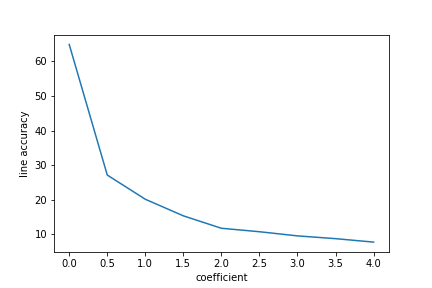
\includegraphics[width=1\linewidth]{pic/accuracy03.png}
		\caption{一元-句准确率}
	\end{minipage}
	\begin{minipage}{0.2\linewidth}
		\centering
		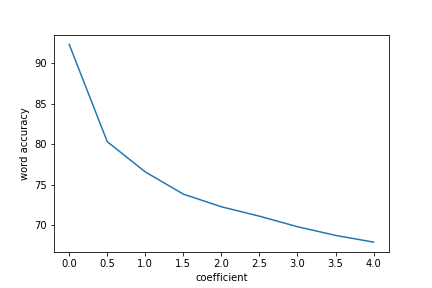
\includegraphics[width=1\linewidth]{pic/accuracy04.png}
		\caption{一元-字准确率}
	\end{minipage}
\end{figure}
	
\begin{figure}[h]
	\centering
	\begin{minipage}{0.2\linewidth}
		\centering
		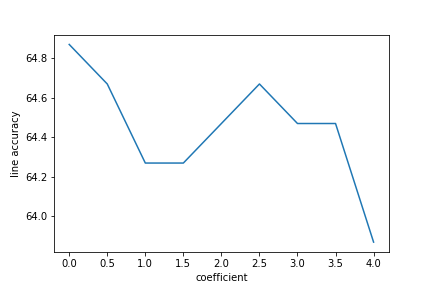
\includegraphics[width=1\linewidth]{pic/accuracy01.png}
		\caption{四元-句准确率}
	\end{minipage}
	\begin{minipage}{0.2\linewidth}
		\centering
		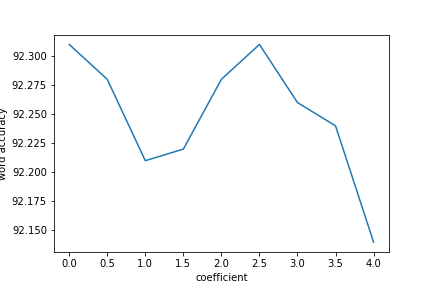
\includegraphics[width=1\linewidth]{pic/accuracy02.png}
		\caption{四元-字准确率}
	\end{minipage}
	
\end{figure}
\subsection{案例分析}
以下是经过参数调整后在标准测试集下模型预测的例子:
\begin{enumerate}
	\item gai zhang hao kai tong jin jin si shi er xiao shi xi fen er shi jiu wan
	
	该账号开通仅仅四十八小时\textbf{吸粉}二十九\textbf{万}
	
	该账号开通仅仅四十八小时\textbf{细分}二十九\textbf{湾}
	\item wei ji bai ke shi yi ge wang luo bai ke quan shu xiang mu
	
	\textbf{维基}百科是一个网络百科全书项目
	
	\textbf{为几}百科是一个网络百科全书项目
	\item gei tong xue men ti gong yi chu xin ling qi xi de tian di
	
	给同学们提供了一\textbf{处}心灵栖息的\textbf{田地}
	
	给同学们提供了一\textbf{初}心灵栖息的\textbf{天地}
	\item chun feng hua yu le wei yang
	
	春风化雨\textbf{乐未央}
	
	春风化雨\textbf{了喂养}
	\item yue gong cong cao cong li tan chu le tou
	
	\textbf{越共}从草丛里探出了头
	
	\textbf{粤工}从草丛里探出了头

\end{enumerate}
\ \\\textbf{总结分析:}
\hspace{1.4em}
\begin{itemize}
	\item 参考正确样例,模型对于不是特别长的句子,甚至是简单古诗文,都能给出正确的结果(针对古诗文的分析将在下一节进一步展开)
	\item 但在一些专有名词(如维基百科、越共)等词,模型不能给出正确结果,这可能和训练集的数据有关,比如训练集中尽管存在一定数量的“\textbf{越共}”词语,但因为报道中一位叫做“\textbf{粤工商}”的通讯员经常出现在新闻标题中,因此“\textbf{粤工}”盖过了“\textbf{越共}”成为这一拼音的首选。再如,\textbf{二十九万}看似是常常出现的数字词语,但原数据集中有高频提及“\textbf{一带九湾}”政策,可能对于模型判断产生了一定的影响。
	\item 而对于另一类错误,如“天地”和“田地”的区别,目前还没有得出很好的解释,甚至从人类视角来看,也很难判断出哪个更接近正确答案。
	\item 目前想到可能的解决办法有:很多问题的产生都可以归结为\textbf{模型局部性过强},而对句子整体的理解不足,因此可以尝试加入词多元模型或者NLP模型,来提高模型对整个句子的理解能力。另外在不改动模型的情况下,如果能\textbf{在数据清洗时过滤掉无关信息}(比如尽管作者名也是文本的一部分,但由于其出现频率过高反而会掩盖其他更关键的信息),模型的准确率可能会得到进一步的提升。
	
	
	
\end{itemize}
\subsection{不同语料库性能对比}
\hspace{1.4em}
新浪新闻2016年的新闻语料库和微博2020年发布的情绪分类技术评测两个语料库来构建的模型存在了 \verb|\model| 目录下,为了测试两种语料库在面对不同类型文本时的表现,除了作业提供的标准测试集外,我还另外构造了两种测试集,测试集内容如下:
\begin{itemize}
	\item 500line: 作业提供的标准测试集
	\item poem: 古诗测试集,选取来自中国古诗文网的文本
	\item semetic: 从微博动态消息中获取的具有口语化和网络流行语特点的文本
	
\end{itemize}
测试结果保存在\verb|\sina|和\verb|\weibo|下

\ \\\textbf{测试结果及分析:}
\begin{figure}[h]
	\centering
	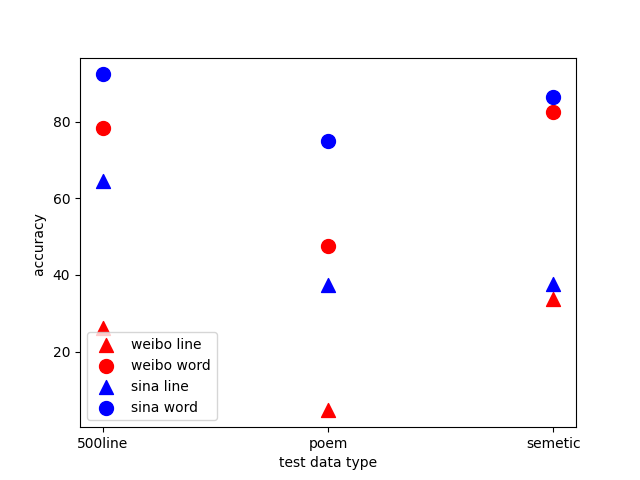
\includegraphics[width=0.8\linewidth]{pic/accuracy05.png}
	\caption{两种语料库在不同测试集上的表现}
\end{figure}
\begin{itemize}
	\item 标准测试集上,\textbf{微博语料库无论是句准确率还是字准确率和新浪语料库均有明显差距}。这也很好理解,微博语料库的规模约为新浪语料库的百分之一,因此在预测准确率上也不如后者。此外,微博语料库中存在大量如 \textbf{“靠他大爷,干啥都不能干的丽丽亮亮的”} 这样具有\textbf{口语}和\textbf{网络用语}特点的文本,由于含有大量表示语气的虚词,在存储信息量上也和以新闻文本为主的新浪语料库存在一定的差距。
	\item 经探索发现,新闻语料库在古诗上预测准确率较高,而微博语料库中由于\textbf{文化类话题}文本较少,对古诗古文相关语句的统计量也不足,因此在古诗训练集上二者的差距明显拉大。下面是一些输出例子:
	\begin {center}
	\begin{tabular}{|c|c|c|}
		\textbf{标准输出} & \textbf{新浪语料库} & \textbf{微博语料库} \\
		\hline
		千里孤坟 & 潜力股份 & 潜力股份 \\
		\hline
		天涯何处无芳草  & 天涯何处无芳草 & 天呀吓出务芳草\\
		\hline
		惊涛拍岸 & 惊涛拍岸 & 经讨拍案 \\
	\end{tabular}
\end{center}
	由于两种语料库收集的主要都是现代语料,因此当拼音对应的某个现代词(如qian li gu fen ->潜力股份)出现频率过高时,两种语料库均无法正确识别。而微博语料库更倾向于将拼音翻译成口语化和网络用语化的结果,这也和我们对该语料库的认识相吻合。
	\item 出于对微博文本特点的考虑,我又从微博中选取了100条左右偏口语化的文本制作成数据集,在该数据集上,两种语料库的预测准确率基本一致。考虑到微博语料库在数量级上的差距,可以说在该任务上,微博语料库效率远大于新浪语料库,相关示例如下
	\begin {center}
	\begin{tabular}{|c|c|c|}
		\textbf{标准输出} & \textbf{新浪语料库} & \textbf{微博语料库} \\
		\hline
		我当年和她结婚真是瞎了眼了 & 我当年和他结婚真是吓了演了 & 我当年和他结婚真是瞎了眼了 \\
		\hline
		妻子想要考验一下自己的老公  & 妻子想要考验一下自己的劳工 & 其子想要考验一下自己的老公\\
	\end{tabular}
\end{center}
可以看出,在“瞎了眼了”、“老公”等常常在网络社交平台出现的词语,微博语料库学习效果更好
\end{itemize}	

综上,在不对任务做限定(对应标准测试集)时,\textbf{语料库规模}对于模型性能起着重要的作用,“大力出奇迹”有其道理。而当面对有特殊限定的任务(比如限定测试集类型)时,合理挑选\textbf{更适配任务的语料库类型},可以起到事半功倍的效果。

\section{收获与感悟}
\hspace{1.4em}
本次输入法实验让我第一次亲自上手了一个人工智能模型,通过这次实现,我对人工智能中的诸多概念,如预测模型、参数调整、训练集与测试集等概念都有了更深入的理解。
本次实验中我得出以下结论:
\begin{itemize}
	\item 更多元的模型会带来更好的效果,但同时也会带来更高的模型训练和运行成本,且在不改变模型算法的条件下,\textbf{仅靠增加模型元数带来的边际收益递减},甚至会带来负收益。
	\item 数学模型仅仅为算法提供了理论依据,在不违背数学理论的大前提下,一些技巧如平滑化、加权平均等策略会起到很好的效果。
	\item \textbf{数据清洗}十分重要,在数据清洗时尝试过滤掉更多杂质信息,对模型性能提升很有帮助
	\item 语料库规模和类型对于模型准确率至关重要,\textbf{选取和任务适配的语料库类型是一种性价比极高的策略}。
\end{itemize}


通过实验和分析,我认为模型可以在以下方面进一步改进:
\begin{itemize}
	\item 尝试引入词多元模型或神经网络,增强模型对整个句子语义的理解
	\item 增加或调整训练数据集,减少模型在新兴用语和专有名词上的知识盲点
\end{itemize}	
	 
本实验中,基于隐Markov模型,我实现了viterbi算法,并在实现该算法的基础上进行模型和参数的优化调整,并针对不同的数据集和测试集效果做了讨论。除此以外,在实验和撰写报告的过程中,我也积累了 python 中的argparse,matplotlib Pyplot等包工具
的使用经验,在此对助教老师的辛苦付出表示感谢!
% End edit to here
%%%%%%%%%%%%%%%%%%%%%%%%%%%%%%%%%%%%%%%%%%%%%%%%%%%%%%%%%%%%%

\end{spacing}
\end{document}

%%%%%%%%%%%%%%%%%%%%%%%%%%%%%%%%%%%%%%%%%%%%%%%%%%%%%%%%%%%%%
